\chapter{多线程 M-JIAJIA 的设计与实现}\label{chap:MJIAJIA}{
    本章主要介绍 M-JIAJIA 的设计与实现,M-JIAJIA 在 JIAJIA 的基础上实现,并继承了域一致性模型,其主要优化集中在通信子系统。
    M-JIAJIA 采用分层模块化设计,解耦通信层和系统核心模块层,两层之间通过消息队列进行通信。
    通信层支持 UDP 通信和 RDMA 通信两种方案,并采用多线程流水化技术优化通信效率。

    \section{设计概览}
    \begin{figure}[!htbp]
        \centering
        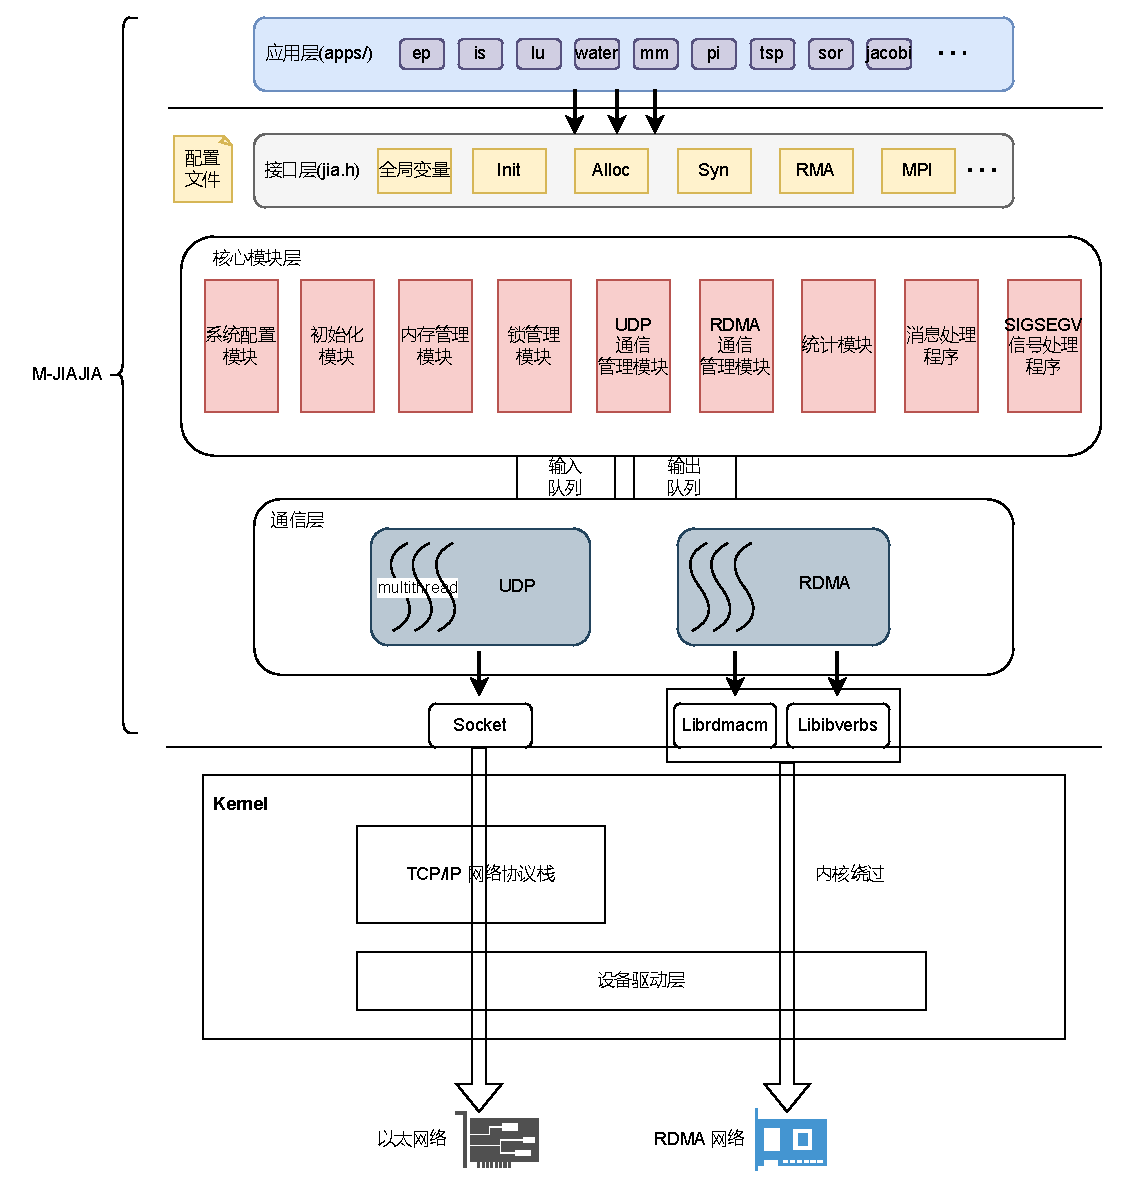
\includegraphics[width=1.0\textwidth]{Img/MJIAJIA系统框架图.drawio.pdf}
        \bicaption{M-JIAJIA系统框架图}{M-JIAJIA Sytem Framework Diagram}
        \label{fig:system-arch}
    \end{figure}
    M-JIAJIA 的整体架构如图~\ref{fig:system-arch} 所示。从上到下依次是应用层、接口层、核心模块层、通信层。
    其中应用层主要包含了 M-JIAJIA 系统的并行测试程序(将在~\ref{chap:experiments}章节做进一步介绍)。
    本章节剩余部分将主要介绍接口层、核心模块层、通信层的设计与实现。

    \section{函数接口设计}
    M-JIAJIA 在函数接口设计上保持了对 JIAJIA 系统接口的兼容,提供列表~\ref{lst:jia-interface}所示 C 语言的编程接口。主要包括全局变量、系统操作、内存操作、同步操作、消息传递接口、和 RDMA(远程内存访问) 接口等。
    \begin{lstlisting}[style=CStyle, caption={M-JIAJIA C 接口总览}, label={lst:jia-interface}]
/* 全局变量 */
extern int jiahosts;
extern int jiapid;
/* 系统操作 */
void jia_init(int argc, int argv);
void jia_exit();
/* 内存操作 */
unsigned long jia_alloc(int totalsize);
unsigned long jia_alloc2(int totalsize, int blocksize);
unsigned long jia_alloc2p(int totalsize, int starthost);
unsigned long jia_alloc3(int totalsize, int blocksize, int starthost);
unsigned long jia_alloc4(int totalsize, int *blocks, int n, int starthost);
unsigned long jia_alloc_random(int totalsize);
unsigned long jia_alloc_array(int totalsize, int *array, int n);
void jia_free(void *addr);
/* 同步操作 */
void jia_lock(int lockid);
void jia_unlock(int lockid);
void jia_barrier();
void jia_wait();
/* 消息传递接口 */
void jia_send(char *buf, int len, int topid, int tag);
int jia_recv(char *buf, int len, int frompid, int tag);
    \end{lstlisting}

    \subsection{配置文件}
    M-JIAJIA 程序采用单程序多数据(Single Program Multiple Data, SPMD)并行计算模式,运行时系统将同一程序动态部署到分布式计算节点上协同执行。
    系统向开发者提供两个配置文件:.jiahosts 和 .jiaconfig,分别用于指定运行的主机和JIAJIA系统的配置。
    同时在JIAJIA系统运行时,每台主机会根据在.jiahosts中的序号拥有自己唯一的jia\_pid。

    \subsection{系统操作}\label{sec:init}
    系统操作接口包含 jia\_init 和 jia\_exit 两个必要接口。jia\_init 用于完成系统的初始化工作,将调用核心层中的初始化模块(图~\ref{fig:mjiajia-init})。
    \begin{figure}[!htbp]
        \centering
        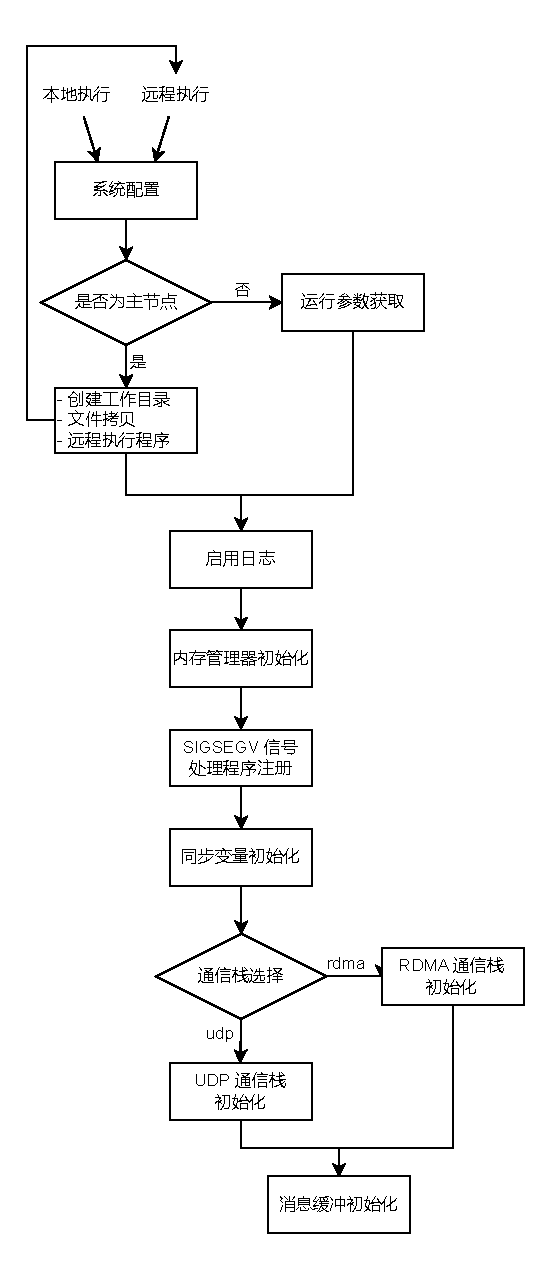
\includegraphics[width=0.6\textwidth]{Img/M-JIAJIA-初始化模块.drawio.pdf}
        \bicaption{M-JIAJIA 初始化模块}{M-JIAJIA initial module}
        \label{fig:mjiajia-init}
    \end{figure}
    相比于 JIAJIA 的初始化模块,M-JIAJIA 做了如下架构改进以满足系统的灵活和可维护性要求:
    \begin{itemize}
        \item 重构配置文件解析逻辑,只依赖 .jiahosts 文件中提供的IP地址、用户名和密码三元组,计算节点之间的连通性由开发者保证。
        \item 引入远程工作目录概念,初始化阶段将为远程节点创建程序工作目录jianode,所有从节点的进程都会在工作目录 jianode 下执行。
        \item 动态初始化网络通信栈,根据系统配置自动选择并初始化 UDP 或 RDMA 通信栈。
    \end{itemize}

    jia\_exit 用于收集所有远程节点的统计信息,并在释放系统资源后退出。
    \subsection{同步操作}
    M-JIAJIA 提供两种同步原语 jia\_lock 和 jia\_barrier 和一种等待原语 jia\_wait,
    用于保证 JIAJIA系统访问共享变量的一致性以及操作的同步性。

    \subsection{消息传递接口}
    消息传递接口用于分布式编程中节点之间的显式通信,M-JIAJIA 支持类消息传递的接口 jia\_send 和 jia\_recv。
    jia\_send 用于向特定主机发送指定数据,而 jia\_recv 负责接收来自其他主机的消息,
    在通信层可以使用 UDP , IPoIB 或 RDMA 通信栈进行通信。

    \newpage
    \subsection{模板与使用说明}
    接口层的介绍将以一个 M-JIAJIA 的模板结束,如列表~\ref{lst:jia-template}所示。利用 M-JIAJIA 接口编程存在两个基本注意点:
    \begin{itemize}
        \item 所有程序均需要以 jia\_init 和 jia\_exit 完成系统的初始化和退出。
        \item 除消息传递接口,锁同步操作外,所有其他接口必须全局执行,不可依赖条件语句。
    \end{itemize}
    \begin{lstlisting}[style=CStyle, caption={M-JIAJIA 应用模板}, label={lst:jia-template}]
#include <jia.h>
int main(int argc, char **argv) {
    jia_init(argc, argv);   // 系统初始化

    jia_alloc(size);
    
    ...  // 共享内存初始化操作

    jia_barrier();  // 同步操作    

    jia_lock(lockid);
    // 临界区操作
    jia_unlock(lockid);
    
    jia_exit(); // 系统退出
    return 0;
}
    \end{lstlisting}

    \section{核心模块设计}
    核心模块层主要由系统的核心处理逻辑组成,负责管理关键数据结构。
    M-JIAJIA的核心模块与JIAJIA基本类似,增加了一个RDMA通信管理模块负责记录网卡参数、
    分配的网卡资源以及连接相关的参数和资源等信息,来进行RDMA通信。

    \section{M-JIAJIA优化设计}
    \subsection{通信栈优化}
    M-JIAJIA 分层设计分离了通信任务和系统任务,系统任务只需与消息队列交互即可完成消息的发送与接收,而通信层负责具体的消息传输。
    通信层支持两种独立的通信协议栈:传统的 UDP 通信栈和 RDMA 通信栈。对于这两个通信栈,M-JIAJIA均作出了相对于JIAJIA的优化设计。

    \subsubsection{UDP 通信栈设计}
    UDP 通信无需建立连接,其核心流程包含三个基本操作:套接字创建、端口绑定及数据收发。M-JIAJIA 系统在运行时需应对高并发通信场景,
    对每台主机使用的端口,多线程通信,以及可靠通信机制提出了更高的要求。对这些方面M-JIAJIA均作出了特定的优化。

    下面将分别介绍 M-JIAJIA UDP 通信栈的端口占用算法、多线程架构设计以及可靠通信实现。
    \begin{enumerate}[label=\arabic*.]
        \item \textbf{端口占用算法设计}

              M-JIAJIA 使用 UDP 协议完成一次通信的过程分为两个阶段:消息的发送与接收,以及确认消息(Ack)的回传与接收。
              根据端口的功能,可以将其划分为发送消息端口、接收消息端口、发送 Ack 端口和接收 Ack 端口。
              不同于 JIAJIA 中为每条UDP通道(每两台之间通信)设置随机的发送消息端口和发送 Ack 端口,M-JIAJIA采用统一的发送消息端口和接收 Ack 端口,
              为每个远端节点设置独立的接收消息端口,同时复用接收消息端口为发送 Ack 端口。

              具体设计如下:在规模为 N 的集群中,每个节点仅使用全局 start\_port 端口基础上[0, N]范围内的端口。
              例如,节点 i 使用 [0, i) 和 (i, N) 范围内的端口接收来自相应节点的消息并回复 Ack,剩余的端口 i 和 N,M-JIAJIA 将使用 i 作为发送端口,
              N 作为接收 Ack 端口。

              通过以上设计,M-JIAJIA 相比 JIAJIA将端口占用复杂度从 $O(N^2)$ 降到 $O(N)$。

              如图~\ref{fig:mjiajia-port-design}所示,图中红线是消息通路,蓝线是Ack通路,采用上述端口设计的host0 和 host2 之间一次通信将执行如下流程:
              \begin{itemize}
                  \item host0 通过 snd\_port 发送消息至 host2 的 port 0 接口端口;
                  \item host2 利用 port 0 作为发送 Ack 端口发送 Ack 至 host0 的 ack\_port。
              \end{itemize}

              图~\ref{fig:mjiajia-comm}是某次UDP通信的端口占用实例。

              \begin{figure}[H]
                  \centering
                  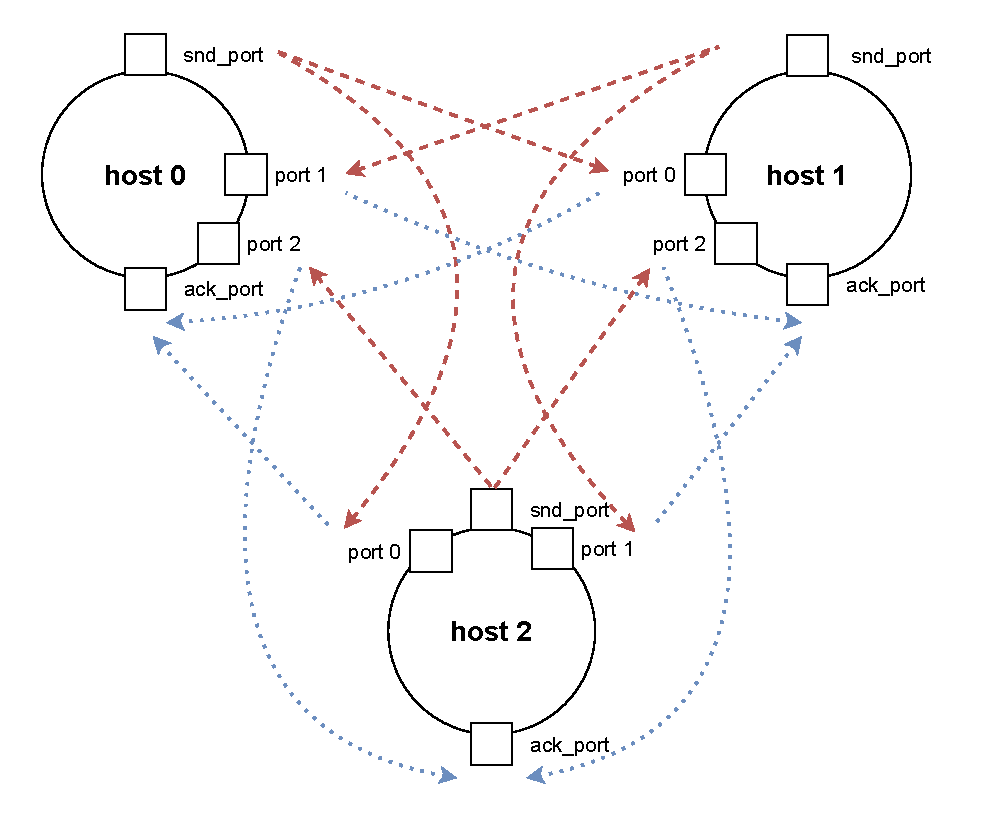
\includegraphics[width=1.0\textwidth]{Img/comm_port.drawio.pdf}
                  \bicaption{端口算法设计示例图}{Example diagram of the port algorithm design}
                  \label{fig:mjiajia-port-design}
              \end{figure}

              \begin{figure}[H]
                  \centering
                  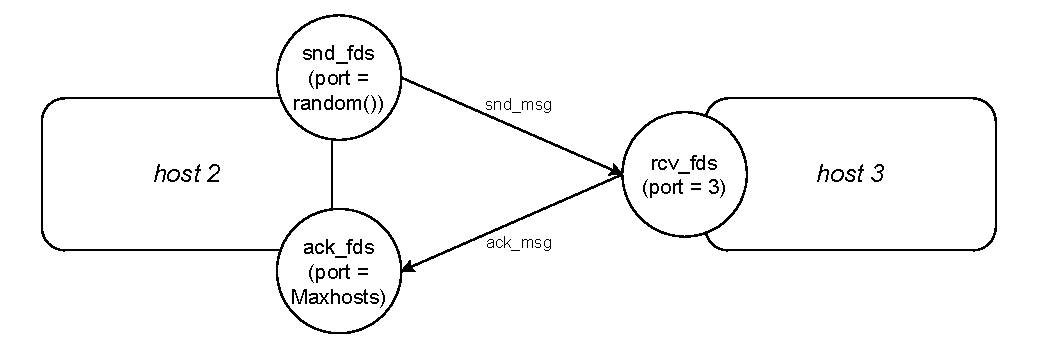
\includegraphics[width=1.0\textwidth]{Img/udp_comm_process.drawio.pdf}
                  \bicaption{UDP单次通信实例}{Example of UDP communication process}
                  \label{fig:mjiajia-comm}
              \end{figure}

        \item \textbf{多线程架构设计}

              在JIAJIA的设计中,使用了SIGIO信号和select组合的多路复用,不过这种方案存在以下不足:
              \begin{itemize}
                  \item SIGIO信号可能在程序执行的任何时刻被触发,需要确保信号处理程序的逻辑是可重入且线程安全的。这涉及到在临界区域处理和返回确认消息时屏蔽信号。
                  \item SIGIO信号是非排队信号,多个 I/O 事件触发信号而信号在处理中被阻塞,后续信号可能丢失。
                  \item 每次信号触发都需要从内核态切换到用户态执行处理函数,频繁的信号涉及大量上下文切换开销。
              \end{itemize}

              为了克服上述缺陷,M-JIAJIA 采用图~\ref{fig:mjiajia-multithread}所示的多线程架构设计。
              该架构将通信任务划分为发送、接收和处理三个子任务,并为每个子任务分配独立线程执行,以提高并发效率。
              \begin{figure}[H]
                  \centering
                  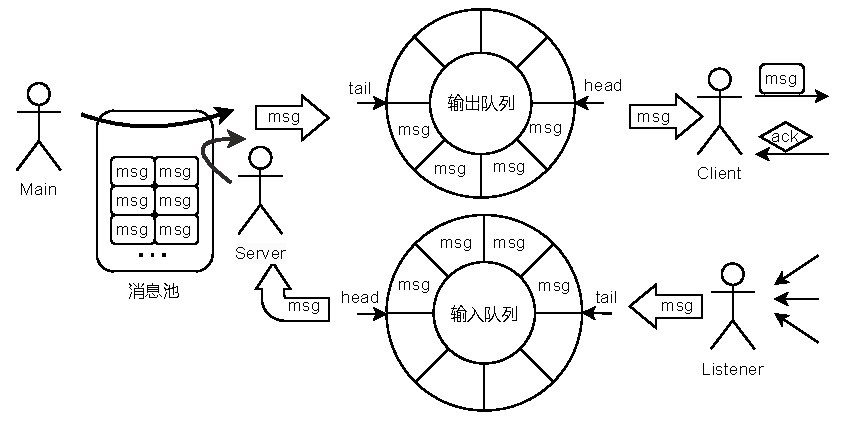
\includegraphics[width=1.0\textwidth]{Img/多线程架构设计.drawio.pdf}
                  \bicaption{\enspace 多线程架构设计}{\enspace Multithread architecture design}
                  \label{fig:mjiajia-multithread}
              \end{figure}

              架构的数据通道依赖于消息池和循环消息队列两个关键数据结构,核心逻辑由发送线程(client)、侦听线程(listener)和服务线程(server)实现。

              \textbf{消息池}:M-JIAJIA在消息池中包含大量预先分配的消息对象,发送消息的线程可以直接从消息池中拿到空闲对象使用,避免频繁分配空间的开销。
              这种设计采用以空间换时间的策略,在高吞吐场景下可以大大提高消息组装的效率;

              \textbf{循环消息队列}:循环消息队列是 M-JIAJIA 核心模块层和通信层之间的通信渠道。
              UDP 通信栈包含输入队列(inqueue)和输出队列(outqueue)两个循环消息队列,分别用于存放接收到的消息和待发送的消息;

              \textbf{发送线程}: 发送线程主要负责检测输出队列是否有待发送的消息,并监听Ack确定消息发送是否成功或需要重传。伪代码如算法~\ref{alg:client-thread} 所示:

              \begin{algorithm}[H]
                  \caption{client thread algorithm}\label{alg:client-thread}
                  \begin{algorithmic}[1] % [1] 使得每行都有行号
                      \Procedure{ClientThread}{}
                      \State initialize $epollfd \gets$ \Call{epoll\_create}{$1$}
                      \State add $epollfd \gets ack\_fds$
                      \While{$true$}
                      \State \Call{sem\_wait}{$outqueue.busy\_count$}
                      \State $msg\_ptr \gets$ \Call{dequeue}{$outqueue$}
                      \For{$retries\_num \gets 0$ to RETRYNUM}
                      \If{$!$ \Call{outsend}{$msg\_ptr$}}
                      \State $break$
                      \EndIf
                      \EndFor
                      \State $snd\_seq[msg\_ptr$->$topid]$++
                      \State \Call{sem\_post}{$outqueue.free\_count$}
                      \EndWhile
                      \State \textbf{return}
                      \EndProcedure

                      \Function{outsend}{$msg$}
                      \If{$msg$->$topid$ = $msg$->$frompid$}
                      \State \textbf{return} \Call{enqueue}{$inqueue,msg$}
                      \Else
                      \State initialize $to\_addr \gets \{msg$->$topid.ip,snd\_port \}$
                      \State \Call{sendto}{$snd\_fds,to\_addr,msg$}
                      \EndIf

                      \While{$true$}
                      \State $nfds \gets$ \Call{epoll\_wait}{$epollfd$}
                      \State \Call{recvfrom}{$ackfds,ack$}
                      \State \textbf{assert}~$\{ack.sid = msg$->$topid\}\;$
                      \State \textbf{assert}~$\{ack.seqno = msg$->$seqno+1\}\;$
                      \State $break$
                      \EndWhile
                      \State \textbf{return} $0$
                      \EndFunction
                  \end{algorithmic}
              \end{algorithm}

              \textbf{侦听线程}:侦听线程负责监视多个接收文件描述符,从就绪的文件描述符中接收消息,将其放入队列,并返回确认消息(Ack)。伪代码如算法~\ref{alg:listen-thread}所示。

              \begin{algorithm}[H]
                  \caption{listen thread algorithm}\label{alg:listen-thread}
                  \begin{algorithmic}[1] % [1] 使得每行都有行号
                      \Procedure{ListenThread}{}
                      \State initialize $epollfd \gets$ \Call{epoll\_create}{$Maxhosts$}
                      \For{$i \gets 0$ to Maxhosts}
                      \State add $epollfd \gets rcv\_fds[i]$
                      \EndFor
                      \While{$true$}
                      \State $nfds \gets$ \Call{epoll\_wait}{$epollfd,events,Maxhosts$}
                      \For{$i \gets 0$ to $nfds$}
                      \State $sockfd \gets events[i].data.fd$
                      \State \Call{recv\_from}{$sockfd,msg$}

                      \State
                      \State $ack \gets \{ msg.seqno+1, msg.topid \}$
                      \State initialize $ack\_addr \gets \{ ack\_port,hosts[msg.frompid].ip \}$
                      \State \Call{sendto}{$sock\_fd,ack\_addr,ack$}

                      \State
                      \If{!\textbf{assert}~$\{msg.seqno = rcv\_seq[to\_id]\}\;$}
                      \State $rcv\_seq[to\_id]$++
                      \State \Call{enqueue}{$inqueue,msg$}
                      \EndIf
                      \EndFor
                      \EndWhile
                      \State \textbf{return}
                      \EndProcedure
                  \end{algorithmic}
              \end{algorithm}

              \textbf{服务线程}:服务线程负责从输入队列中提取消息,并根据消息类型进行相应的服务。伪代码如算法~\ref{alg:server-thread} 所示。
              \begin{algorithm}[H]
                  \caption{server thread algorithm}\label{alg:server-thread}
                  \begin{algorithmic}[1] % [1] 使得每行都有行号
                      \Procedure{ServerThread}{}
                      \State \Call{sem\_wait}{$inqueue.busy\_count$}

                      \State $msg\_ptr \gets$ \Call{dequeue}{$inqueue$}
                      \State \Call{msg\_handle}{$msg\_ptr$}

                      \State \Call{sem\_post}{$inqueue.free\_count$}
                      \State \textbf{return}
                      \EndProcedure
                  \end{algorithmic}
              \end{algorithm}

        \item \textbf{可靠通信实现}

              针对 UDP 协议无连接、不可靠的传输特性,M-JIAJIA 系统在应用层采用消息序号、确认与超时重传机制实现可靠通信,见图~\ref{fig:mjiajia-reliable-comm}。

              \textbf{消息序号}:消息序号用于确保通信的有序性。通信管理器维护与每个远端节点通信的当前消息序号,发送线程从输出队列中获取消息后,将据此为消息分配序号。

              \textbf{确认消息}:每当接收到一条消息,侦听线程会生成并返回相应的确认消息(Ack)。Ack由两部分组成:期望接收的下一个消息的序号以及本机标识。

              \textbf{超时重传机制}:发送线程在发送消息后进入阻塞状态,等待 Ack 消息。如果超时未收到 Ack,则触发重传机制。然而,对于不匹配的 Ack,系统仅忽略处理,不触发重传。
              \begin{figure}[H]
                  \centering
                  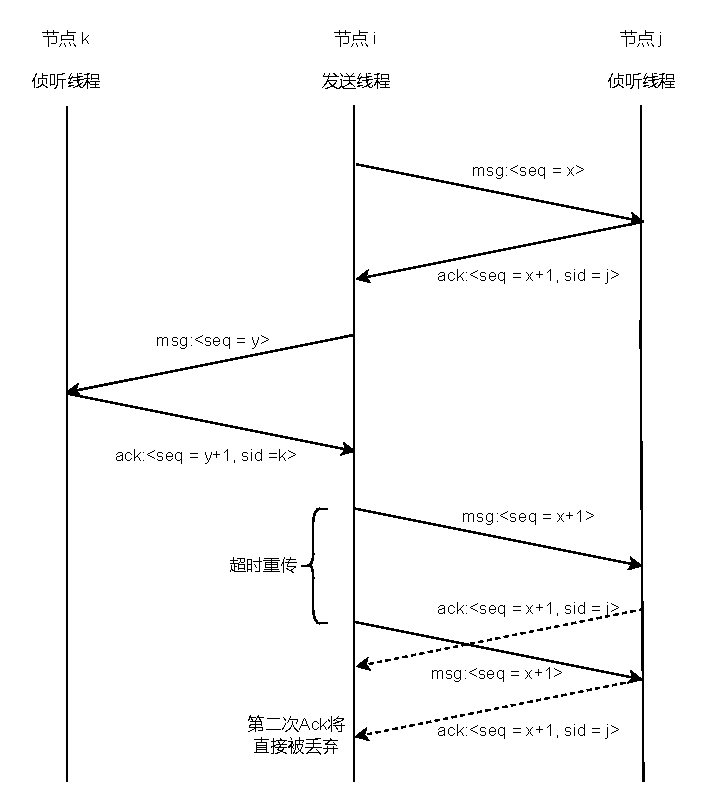
\includegraphics[width=1\textwidth]{Img/M-JIAJIA 可靠通信实现.drawio.pdf}
                  \bicaption{\enspace M-JIAJIA 可靠通信实现}{\enspace M-JIAJIA Reliable Communication Implementation}
                  \label{fig:mjiajia-reliable-comm}
              \end{figure}

    \end{enumerate}

    \subsubsection{RDMA 通信栈设计}
    RDMA 通信模块包含 RDMA 通信栈的设计与实现,这部分将在第~\ref{chap:RJIAJIA}章节介绍。

    \subsection{远程预取优化}
    对于软件 DSM 系统而言,远程内存访问开销是通信开销的重要组成部分,也是影响系统性能的关键因素之一。
    尽管 RDMA 高速网络显著降低了通信延迟,但远程内存访问的开销仍比本地内存访问高 1 至 2 个数量级~\citep{cai2018gam}。
    为此,远程预取技术被广泛研究和应用,以优化数据访问模式,减少远程访问延迟,从而提升系统整体性能。

    M-JIAJIA 的缓存策略是将远端页缓存至本机相同的虚拟地址空间,即共享地址为 addr 的远端页将在本机的 addr 虚拟地址上进行缓存。

    M-JIAJIA 的预取策略是在远程取页时,提前获取远端节点上分配的后续几页共享页,缓存至本地并赋予读权限,从而提升访问效率。

    具体实现方案依赖于三个变量:预取开关(prefetch)、预取页数(prefetch\_pages)和最大检查页数(max\_checking\_pages)。预取的触发条件是:
    $$
        \left\{
        \begin{aligned}
             & \texttt{prefetch = on},           \\
             & \texttt{prefetch\_pages > 0},     \\
             & \texttt{max\_checking\_pages > 0}
        \end{aligned}
        \right.
    $$

    在启用预取的情况下,远端节点在接收到读取页请求后,将最多向后检查 max\_checking\_pages 相邻页是否是共享页,并至多打包 prefetch\_pages 页一同返回。预取优化的效果取决于两次消息传递获取写权限的模式出现的概率以及共享内存的分配策略。若采用循环页分配算法,使相邻页分配至不同节点,预取优化的效果将受到限制。


    \subsection{其他优化}
    \begin{itemize}
        \item M-JIAJIA 优化了 .jiahosts 的处理逻辑,仅依赖 IP 地址、用户名和密码三元组,无需依赖系统配置文件 /etc/hosts;
        \item M-JIAJIA 引入了 .jiaconf 配置文件,以支持自定义系统通信环境和资源管理;
        \item M-JIAJIA 引入了分级日志机制,以满足不同详细程度的调试需求。
    \end{itemize}

    \section{本章小结}
    本章 3.1 节给出 M-JIAJIA 系统的整体框架图,简要介绍了其基本层次结构。

    本章 3.2 节主要介绍 M-JIAJIA 的函数接口。包括配置文件,系统的基本操作和使用说明。

    本章 3.3 节介绍了 M-JIAJIA 的核心模块设计,相比JIAJIA增加了一个RDMA通信模块。

    本章 3.4 节介绍了 M-JIAJIA 相比JIAJIA的一些优化,包括通信栈优化,远程预取优化等。
}
